\chapter{Introduction}
\newcommand{\ordre}{\textbf{Ordre}}
\newcommand{\direction}{\textbf{Direction}}
\newcommand{\nnn}{\textbf{NaturelNonNul}}
\newcommand{\Labyrinthe}{\textbf{Labyrinthe}}
\newcommand{\cdc}{\textbf{ChaineDeCaracteres}}

Dans le cadre de nos études en troisième année à l'INSA Rouen Normandie au sein du département ITI, nous avons reçu l'opportunité de participer au projet Integratif Smart Robot. Celui-ci vise à renforcer et développer des compétences que nous avons abordé en cours. Notre objectif était de concevoir un robot capable de sortir le plus rapidement possible d’un Labyrinthe de forme carré, en suivant une ligne pour se guider.

\section{Différentes compétences}
Ce projet se compose notamment de deux grandes parties, celles-ci nécessitant des compétences en algorithmique et en électronique.
Nous nous sommes appuyés sur les outils suivants pour réaliser ce projet:
\begin{itemize}
    \item \texttt{Doxygen} pour la génération de la documentation du code.
    \item \texttt{Fritzing} pour la conception du circuit électronique.
    \item \texttt{GitLab} pour le partage du code source et la création de tickets des actions et demandes.
    \item \texttt{Make} pour la compilation du code source.
    \item \texttt{LaTeX} pour générer un rapport de projet en .pdf après compilation.
\end{itemize}
\subsection{Algorithmique}
Tout d'abord, la partie algorithmique permet de créer un algorithme et de l'implémenter permettant de trouver le chemin le plus court pour sortir du labyrinthe. Cette implémentation est le résultat de différentes étapes du cycle en V, celles-ci sont détaillés dans la suite du rapport.
\subsection{Électronique}
La partie électronique a pour but de concevoir le robot qui va utiliser l'algorithme pour sortir du labyrinthe. Ainsi, cela nous a poussé à la réflexion du placement des différents composants sur le robot. Cette conception a fait appel à différentes compétences, comme la création d'un schéma électronique et son câblage associé, le codage sur carte Raspberry, la soudure ...
\vspace{5mm}

\section{Organisation du travail}

L'outil GitLab permet le partage du code dans le groupe mais propose également la création de tickets pour suivre les modifications. Ainsi, nous avons créé les tickets suivants afin d'effectuer les tâches requises par le projet. Chaque ticket sera référencé par un \# suivit de son numéro (le numéro suit l'ordre de création des tickets): 
\vspace{2mm}

\begin{itemize}
    \item \#2: ce qui concerne latex.
    \item \#3: ce qui concerne les TADs.
    \item \#4: ce qui concerne l'analyse descendante (partie algorithmique/\\ électronique).
    \item \#5: ce qui concerne le schéma électrique et le fritzing.
    \item \#6: ce qui concerne la conception préliminaire et la conception détaillée.
    \item \#7: ce qui concerne la fonction creerLabyrinthe.c.
    \item \#8: ce qui concerne la fonction analyseFichier.c.
    \item \#9: ce qui concerne la fonction resolutionLabyrinthe.c.
    \item \#10: ce qui concerne le code du robot.
    \item \#11: ce qui concerne tous les types.c.
    \item \#12: ce qui concerne les tests unitaires.
    \item \#13: ce qui concerne les makefiles.
    \item \#14: ce qui concerne l'espace de nommage.
    \item \#16: ce qui concerne la documentation de la partie électronique.
    \item \#17: ce qui concerne les tests sur le robot.
    \item \#18: ce qui concerne le script bash.
\end{itemize}
\vspace{5mm}

Les tickets étaient ainsi à disposition de chaque membre du groupe afin d'assurer la bonne organisation du projet et le suivi des tâches. Cependant, pour assurer le bon déroulement du projet, la répartition du travail était indiqué par le chef de projet. Ainsi, chaque membre du groupe s'est vu attribuer différentes tâches tout au long du projet. En cela, chaque membre du groupe a pu travailler sur différents aspects du projet:

\begin{itemize}
    \item \textbf{Delaplace Yohann}\\
    développement des makefile, bash et tests unitaires,\\
    rédaction du rapport latex.
    \item \textbf{Lenoble Louis (chef de projet)}\\
    organisation du projet,\\
    montage du robot,\\
    développement de la partie algorithmique.
    \item \textbf{Planchot Maël}\\
    développement de la partie électronique et Doxygen.
    \item \textbf{Sanson Dylan}\\
    développement de la partie algorithimique et électronique.
    \item \textbf{Sourdrille Nathan}\\
    développement de la partie algorithmique et électronique,\\
    rédaction du rapport latex et bilan de chaque séance.
    
\end{itemize} 
\vspace{0.5cm}

\textbf{Planning :}\\
Afin de maintenir un bon rythme de travail et de pouvoir mener le projet à son terme, nous avons mis en place un planning qui respecte les critères suivants: 
\begin{itemize}
\item {Les tâches à faire avant la séance}
\item {Les tâches à faire durant la séance}
\item {Le déroulement de la séance}
\item {Le bilan de fin de séance}
\end{itemize} 
\vspace{0.5cm}
Voici, par exemple, le planning concernant les séances d'électronique :

\begin{figure}[h!]
    \hspace{-2cm}
    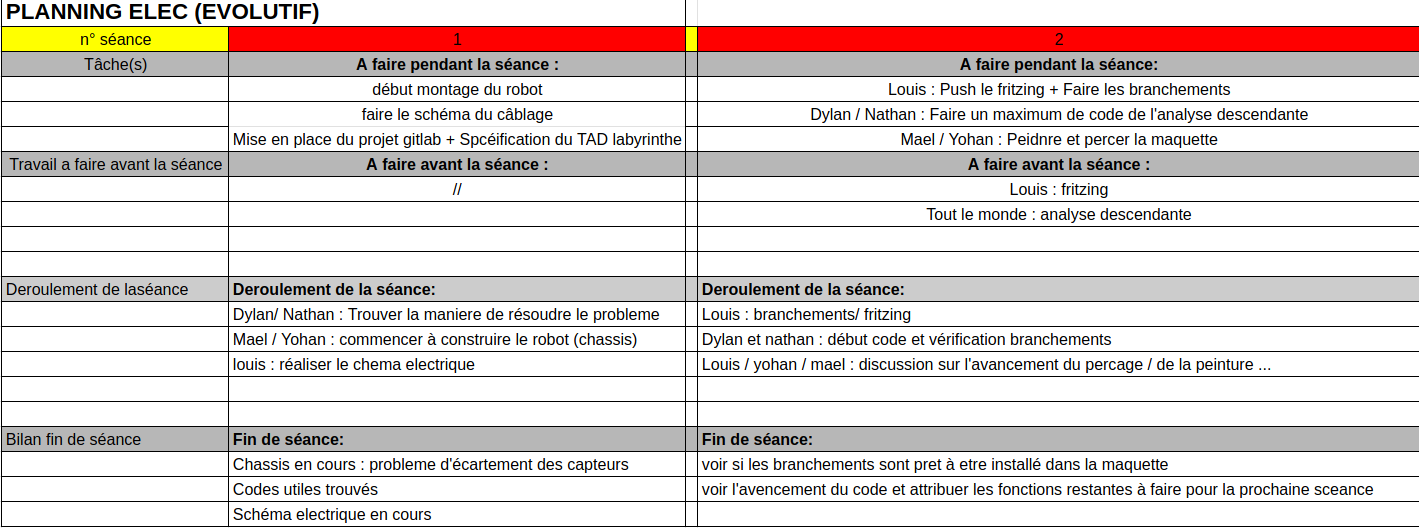
\includegraphics[width=1.2\textwidth]{imagesRapport/planning1.png}
    \caption{planning séances 1 et 2}
    \label{fig:exemple}
\end{figure}
\begin{figure}[h!]
    \hspace{-2cm}
    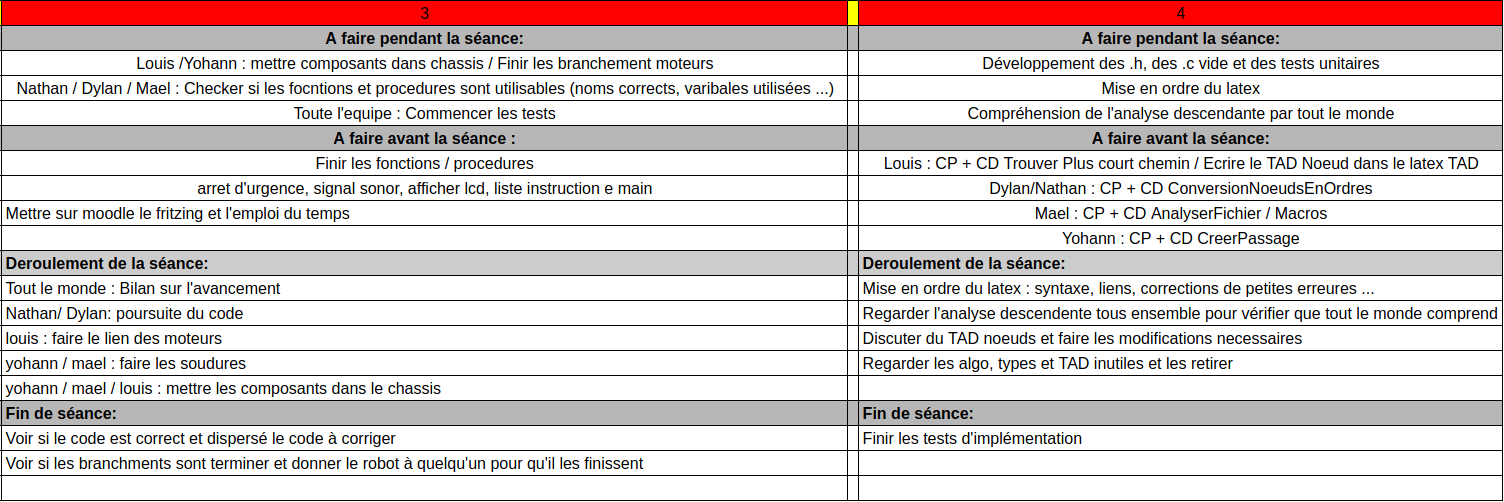
\includegraphics[width=1.2\textwidth]{imagesRapport/planning2.png}
    \caption{planning séances 3 et 4}
    \label{fig:exemple}
\end{figure}
\vspace{5cm}

\textbf{Matrice des tâches réalisées}\\
Afin de mieux visualiser l'implication de chaque membre du groupe dans les différentes étapes du projet, ci-dessous est présenté la matrice des tâches réalisées (le niveau d'implication dans chaque tâche est indiqué via un pourcentage) :
\begin{table}[ht]
\begin{adjustwidth}{-3cm}{-3cm}
\centering
\begin{tabular}{|p{2.2cm}|p{2.2cm}|p{2.2cm}|p{2.2cm}|p{2.2cm}|p{2.2cm}|}
\hline
\textbf{Tâches} & \textbf{Delaplace Yohann} & \textbf{Lenoble Louis} & \textbf{Planchot Maël} & \textbf{Sanson Dylan} & \textbf{Sourdrille Nathan} \\
\hline
schéma électronique fritzing & 0 & 100 & 0 & 0 & 0 \\
\hline
choix du placement des capteurs & 20 & 20 & 20 & 20 & 20 \\
\hline
création des TAD & 20 & 20 & 20 & 20 & 20 \\
\hline
analyse descedante & 20 & 20 & 20 & 20 & 20 \\
\hline
recherche algorithme de résolution & 0 & 33 & 33 & 33 & 0 \\
\hline
conception détaillée des fonctions principales & 0 & 33 & 33 & 33 & 0 \\
\hline
développement des .h (algo) & 0 & 65 & 0 & 25 & 10 \\
\hline
développement des .h (élec) & 0 & 0 & 50 & 50 & 0 \\
\hline
développement des .c (types) & 0 & 50 & 0 & 20 & 30 \\
\hline
développement des .c (algo) & 20 & 40 & 0 & 40 & 0 \\
\hline
développement des .c (élec) & 0 & 0 & 60 & 30 & 10 \\
\hline
tests unitaires (algo) & 90 & 0 & 0 & 5 & 5 \\
\hline
tests unitaires (élec) & 20 & 20 & 20 & 20 & 20 \\
\hline
tests d'intégration (algo) & 0 & 50 & 0 & 50 & 0 \\
\hline
tests d'intégration (élec) & 20 & 10 & 50 & 10 & 10 \\
\hline
makefile & 90 & 0 & 10 & 0 & 0 \\
\hline
bash & 100 & 0 & 0 & 0 & 0 \\
\hline
mise en place de doxygen & 0 & 0 & 100 & 0 & 0 \\
\hline
documentation & 0 & 33 & 33 & 33 & 0 \\
\hline
mise en place du latex & 50 & 0 & 50 & 0 & 0 \\
\hline
rapport latex & 25 & 5 & 0 & 0 & 70 \\
\hline

\end{tabular}
\end{adjustwidth}
\end{table}

